En este capítulo se presentan los conceptos sobre los cuales se basa el trabajo así como definiciones relativas al problema y algunos algortimos específicos relevantes para el presente trabajo.
\section{Optimización}
La optimización es una herramienta que nos ayuda a encontrar \textit{la mejor} entre diferentes opciones elegibles. En nuestra vida diaria a menudo nos encontramos en este tipo de situaciones, por ejemplo al elegir entre diferentes rutas para llegar a algún lugar o entre diferentes productos.\\

En lenguaje matemático un problema de optimización consiste en minimizar o maximizar una función que le asigna un valor a cada una de las opciones que tenemos disponibles. Para la definición formal se adopta la siguiente notación:
\begin{itemize}
    \item $X$ El conjunto de opciones o soluciones disponibles.
    \item $f:X\rightarrow \mathbb{R}$ La función objetivo a minimizar o maximizar.
\end{itemize}
El problema consiste en hallar:
\begin{gather}
\min_{x\in X} f(x)
\end{gather}
Es importante mencionar que cualquier problema en el que se requiera encontrar el argumento que hace tomar el valor máximo a $f$ puede transformarse en un problema equivalente de minimización con el reemplazo $f(x) \leftarrow -f(x)$, por lo que puede considerarse solo el caso de minimización sin pérdida de generalidad.\\

De acuerdo con la definición del problema como tal o con los métodos de solución se distinguen distintas ramas de la optimización. A continuación se presentan algunas de ellas de especial importancia para el presente trabajo.

\subsection*{Optimización con restricciones}
A la definición de un problema de optimización también pueden agregarse un conjunto de restricciones las cuales son en la práctica un conjunto de funciones que toman una solución e indican si esta cumple o no con ellas, se dice que una solución es factible si cumple con las restricciones e infactible en caso contrario. Estas restricciones se agregan ya sea porque el problema así lo requiere o bien para asegurarse que la solución tenga sentido, por ejemplo si $f$ tiene como argumento un número real que representa una longitud debe requerirse que esta longitud sea un número positivo.\\

\subsection*{Optimización global y local}

Hallar el mínimo de la función sobre todo el conjunto $X$ recibe el nombre de optimización global, esto puede llegar a ser muy costoso o incluso imposible de obtener por lo que es común optar por obtener un mínimo local, es decir, una solución que sea la mejor de un subconjunto de $X$. A menudo este subconjunto se define utilizando alguna medida de distancia entre soluciones y considerando a todas las soluciones que estén en algún rango de distancia a otra de referencia o bien añadiendo un operador que permita crear soluciones nuevas a partir de una solución ya conocida. \\

\subsection*{Optimización estocástica}
También puede ser que el algoritmo planteado para resolver el problema de optimización sea no determinista i.e. puede obtener soluciones diferentes aunque tenga las mismas condiciones iniciales. En muchas ocasiones es ventajoso tener algo de aleatoriedad porque nos permite explorar el espacio de búsqueda con pocos sesgos. Estos métodos son especialmente útiles cuando el espacio de búsqueda es poco <<predecible>> en el sentido en que no podemos a priori distinguir regiones de buena o mala calidad. Tal vez el método más famoso de este tipo es el llamado recocido simulado, el cual se inspira en un fenómeno metalúrgico y que encuentra soluciones muy buenas a una gran variedad de problemas de optimización.

\subsection*{Optimización continua y discreta}
 En la definición anterior no se requiere que el conjunto de soluciones tenga alguna propiedad o alguna estructura adicional. Por ejemplo el conjunto de soluciones puede ser un conjunto numerable ( e.g. los enteros ) o no numerable ( e.g. los números reales ). Estos dos casos dividen a la optimización en dos ramas: optimización continua y optimización discreta. En general los problemas de optimización continua suelen ser más fáciles de abordar\cite{nocedal2006numerical} porque en muchas ocasiones es posible obtener información del valor de la función objetivo de puntos cercanos a cierto punto conocido mientras que en los problemas discretos esto rara vez puede hacerse.\\

\subsection*{Optimización combinatoria}
Dentro de los problemas de optimización discreta se distinguen los problemas de optimización combinatoria. Formalmente un problema de optimización combinatoria consta de los siguientes elementos\cite{Blum2003}:
\begin{itemize}
    \item Un conjunto de variables $Z=\{z_1,z_2,...,z_n\}$
    \item Dominio para cada variable $D_1,D_2,...,D_n$
    \item Restricciones entre variables
\end{itemize}

En muchos problemas de optimización combinatoria el conjunto de soluciones no tiene alguna estructura adicional que ayude a buscar el mínimo de la función objetivo; es raro que exista un ordenamiento de las soluciones o una medida de distancia entre ellas que brinde propiedades a la función objetivo tales como continuidad o suavidad las cuales facilitarían la búsqueda del mínimo. Dicho de otro modo, no tenemos a priori una forma eficiente de explorar el espacio de búsqueda. Ante estas limitaciones surgieron técnicas conocidas como metaheurísticas que buscan facilitar la resolución de estos problemas.

\section{Metaheurísticas}
Es muy común que en nuestra cotidianidad nos enfrentemos a problemas tan difíciles o para los que tengamos tan poco tiempo de decisión que no podamos hacer un análisis riguroso, en estos casos es muy común que utilicemos algún método (posiblemente basado en la experiencia) que nos permita hallar una solución aceptable, por ejemplo, es común que reemplacemos el problema por uno más simple que sí podemos responder y cuya respuesta está relacionada con nuestro problema original (no podemos predecir con certeza si lloverá durante el día pero sí podemos responder si el cielo está plagado de nubes oscuras).

En el contexto de la optimización una metaheurística es una metodología de alto nivel que combina diferentes heurísticas y puede aplicarse para resolver de manera aproximada una gran cantidad de problemas. En la práctica existen numerosas metaheurísticas que pueden ser muy diferentes entre sí por lo que no hay un sistema de clasificación universalmente aceptado aunque se han propuesto diferentes criterios de clasificación \cite{Stegherr2020} así como características como:
\begin{itemize}
\item De trayectoria vs discontinua. Una metaheurística de trayectoria consiste en, dada una solución inicial, mejorarla de manera iterativa mediante algún operador que <<mueve>> a la solución a través del espacio de búsqueda %extender.
\item Basadas en población vs basadas en una sola solución. En las metaheurísticas basadas en población se mantiene un conjunto de soluciones candidatas.
\item Basadas en búsqueda local vs constructivas. Como se explicará más adelante, en la búsqueda local, el proceso de mejora implica la evaluación de soluciones muy parecidas a una solución inicial dada mientras que en las constructivas se crean nuevas soluciones de acuerdo a una heurística o algoritmo preestablecido.
\item Con uso de memoria vs sin uso de memoria. El uso de memoria consiste en almacenar información que nos ayude a explorar el espacio de búsqueda, por ejemplo una lista de soluciones previamente visitadas.
\end{itemize} 
Los primeros dos de estos criterios están muy relacionados porque casi todas las metaheurísticas discontinuas son poblacionales y muchas de trayectoria son basadas en una sola solución.


Si bien las metaheurísticas son muy diversas existen elementos comunes que tienen un papel determinante en el buen funcionamiento de las mismas. En específico para las metaheurísticas de trayectoria existen tres conceptos que determinan el llamado paisaje de búsqueda: las soluciones en sí, la forma en que las soluciones están conectadas y cómo podemos compararlas entre sí. A continuación se describe cada uno de ellos.
% introducir los conceptos siguientes
\subsection{Representación}
Puede ser que el problema de optimización en el que estemos interesados surja directamente de las matemáticas aunque si estamos interesados en un problema de nuestro entorno físico es necesario que tengamos que idear una forma de traducirlo a un lenguaje matemático, incluidas las soluciones al mismo. Debemos encontrar una forma de representar de manera útil las soluciones posibles.
Por ejemplo si buscamos un ordenamiento óptimo para algún conjunto de $n$ cosas podemos asignarle a cada elemento del conjunto un número entero del $1$ al $n$, en este modelo el espacio de soluciones está constituido por todas las permutaciones de los números del $1$ al $n$. 

Hay varias maneras de representar permutaciones, podemos usar un arreglo de $n$ entradas o bien una matriz de permutación por mencionar algunos. Algo sumamente importante es que estas dos formas de representar las soluciones son muy distintas y se tiene que trabajar con ellas de manera muy diferente. La primera de ellas puede llegar a representar \textit{soluciones no factibles} por ejemplo que aparezca un número repetido, mientras que la segunda no.

Con el ejemplo anterior también podemos ver que si queremos establecer algunos operadores que, por ejemplo, perturben la solución tendremos que definirlos de maneras completamente distintas. También es importante notar que es posible que el número de soluciones no factibles que podamos representar sea mayor que el de las factibles.

Formalmente una representación es un mapa que asocia elementos entre el conjunto de soluciones y el conjunto de las representaciones. Este mapeo no tiene por que ser suryectivo, es decir que puede ser que solo asigne una representación a parte del conjunto de soluciones. También puede ser el caso como se mencionó anteriormente que haya representaciones que no correspondan a soluciones. Pueden distinguirse tres tipos de representaciones\cite{Cheng1996} de acuerdo a como asocian los elementos de estos dos conjuntos.
\begin{itemize}
    \item $1$ a $1$ A cada solución le corresponde una única representación.
    \item $1$ a $n$ La misma representación puede asociarse a varias soluciones.
    \item $n$ a $1$ Una solución puede tener diferentes representaciones.
\end{itemize}

\begin{figure}[H]
    \centering
    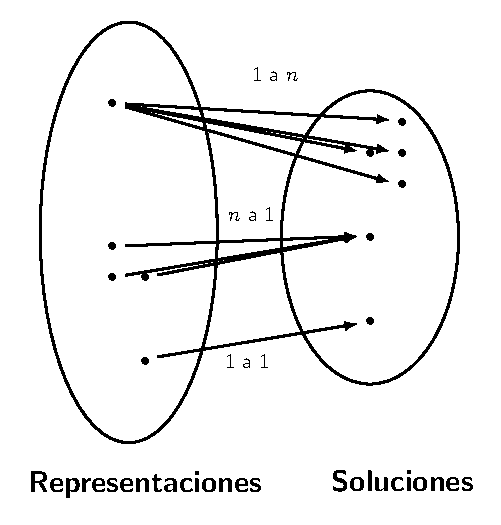
\includegraphics[scale=1]{Imagenes/representacion.pdf}
    \caption{Tipos de representaciones}
\end{figure}

Lo más conveniente suele ser un mapeo $1$ a $1$ porque resulta mucho más eficiente y lo menos deseable es tener un mapeo $n$ a $1$ en el que es posible que la misma representación esté asociada a soluciones de calidad muy diferente. 


\subsection{Vecindad}
La definición de vecindad es crucial para las metaheurísticas de trayectoria y las basadas en una sola solución.
Formalmente, una vecindad es un mapeo $N:X\rightarrow 2^X$ que le asigna a cada solución $x\in X$ un subconjunto de soluciones en $X$. Intuitivamente podemos pensar que es una forma de definir a las soluciones que <<rodean>> a otra. Se dice que la solución $y$ es un vecino de $x$ si $y\in N(x)$.

A partir de la definición de vecindad podemos también definir un operador de movimiento $M:X\rightarrow X$ cuyo efecto al aplicarlo a una solución sea transformarla en una que pertenezca a su vecindad, i.e. este operador selecciona a un vecino de la solución inicial.  
\[M(x)=y\in N(x)\quad x\neq y\]

\subsection{Función de aptitud o fitness}
Aunque para un problema de optimización ya se tiene definida una función objetivo que se quiere minimizar, no siempre tenderemos el mejor desempeño de las metaheurísticas con solo esta función por lo que resulta benéfico plantear una nueva función a minimizar con la que tengamos mejor desempeño. Por ejemplo puede suceder que aunque dos soluciones tengan asociado el mismo valor de la función objetivo una de ellas posee características que la hacen un mejor punto de partida para alguna metaheurística.

Esta función debe asociar a cada solución un elemento de un conjunto donde esté definido un ordenamiento total. En esencia esta función define un operador de comparación entre soluciones de modo que podemos elegir la mejor de dos soluciones.\\

\subsection{Paisaje de búsqueda}

Una vez que tenemos el espacio de búsqueda y operadores de cambio para generar nuevas soluciones a partir de otras, se define el espacio de búsqueda como un grafo dirigido $G$ en el que los nodos son las soluciones al problema y una solución $x$ está conectada a otra $y$ si podemos generar a $y$ aplicando los operadores de cambio a $x$.

Podemos asociar a cada solución en el espacio un valor de aptitud o fitness que mide la calidad de dicha solución. La adición de esta función de aptitud al espacio de búsqueda genera al paisaje de búsqueda. Formalmente el paisaje de búsqueda $\mathcal{L}$ es entonces una tupla conformada por el espacio de búsqueda junto con una función objetivo que guía la búsqueda $\mathcal{L}=(G,f)$

A continuación se muestra una representación pictórica de la definición del paisaje de búsqueda para un problema de optimización.
\begin{figure}[H]
\begin{subfigure}{.4\textwidth}
    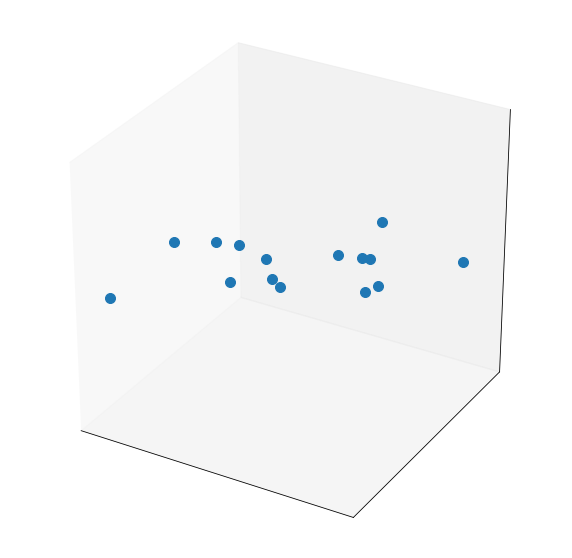
\includegraphics[scale=.5]{Imagenes/search1.png}
    \caption{Soluciones representables}
\end{subfigure}
\begin{subfigure}{.5\textwidth}
    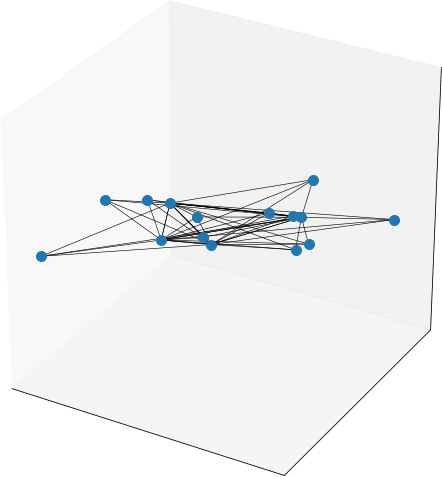
\includegraphics[scale=.5]{Imagenes/search2.png}
    \caption{Relaciones inducidas por los operadores de cambio}
\end{subfigure}
\begin{subfigure}{\textwidth}
    \centering
    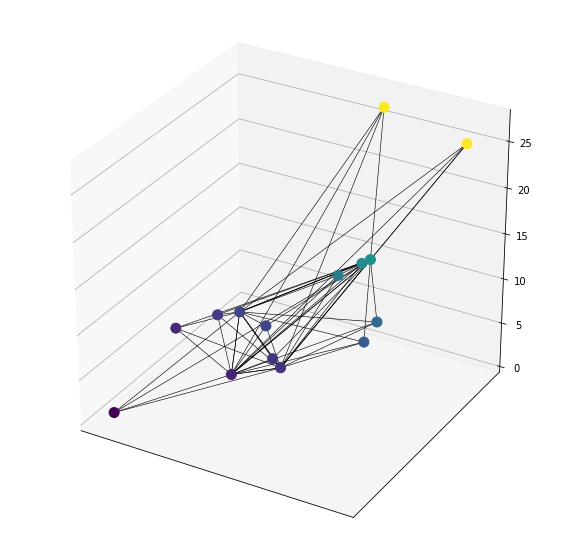
\includegraphics[scale=.5]{Imagenes/search3.png}
    \caption{Adición de la función de fitness}    
\end{subfigure}
\label{fig:landscape}
\caption{Creación del paisaje de búsqueda}
\end{figure}

El paisaje de búsqueda es el <<terreno>> a explorar y puede cambiar si cambiamos cualquiera de sus componentes, podría ser que alguna representación nos centre en un subconjunto de soluciones convenientes o que alguna estructura de vecindad se proponga de modo que las mejores soluciones nunca están muy lejos del resto, o que la función de fitness nos ayude a atravesar cúmulos de soluciones que serían iguales sin ella.

La estructura del paisaje de búsqueda influye de manera determinante en el éxito o fracaso de las metaheurísticas. Dependiendo de la <<forma>> que tenga el paisaje se favorecerá el uso de ciertas metaheurísticas. La <<forma>> del paisaje hace referencia a cómo cambia el valor de fitness para soluciones conectadas entre sí. Dos medidas que son generalmente utilizadas para esto miden cómo cambia el valor de la función de fitness conforme nos acercamos a un óptimo local y la otra mide qué tanto cambia el fitness entre soluciones vecinas\cite{skauffman}. La primera de estas medidas nos da una idea de qué tan grandes son los valles que rodean a un mínimo local si es que existen y la segunda nos da una ida de la rugosidad del paisaje.

% imagen
\begin{figure}[H]
\begin{subfigure}{.45\textwidth}
    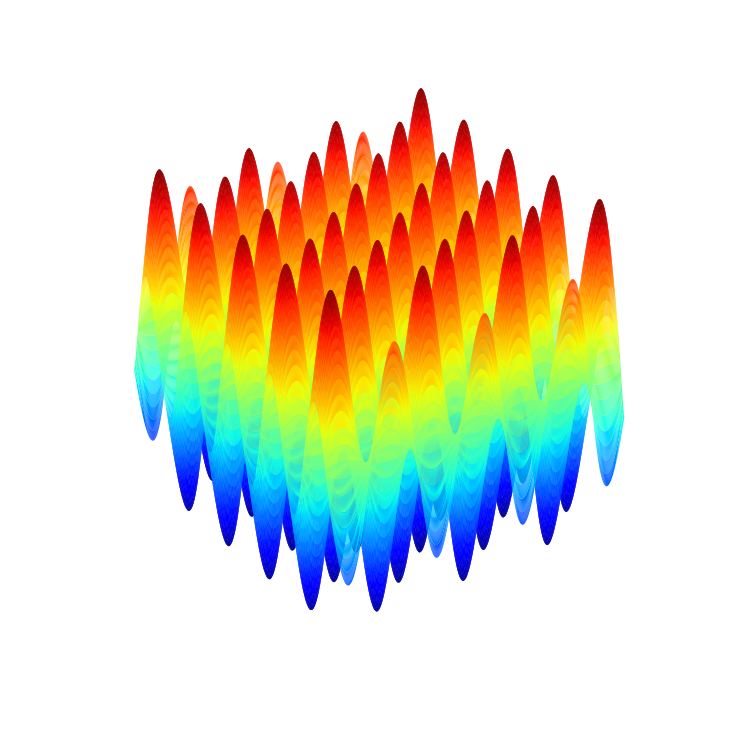
\includegraphics[scale=.4]{Imagenes/rugged.png}
    \caption{Paisaje rugoso con muchos óptimos locales}
\end{subfigure}
\begin{subfigure}{.5\textwidth}
    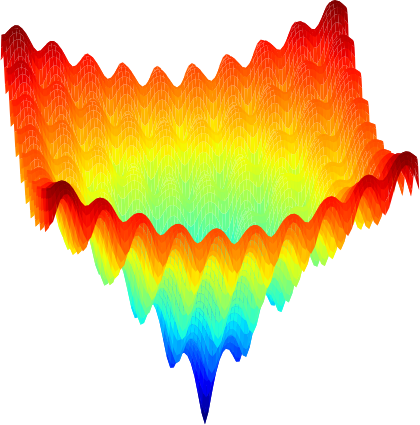
\includegraphics[scale=.4]{Imagenes/ruggedvalley.png}
    \caption{Paisaje rugoso con con un gran valle}
\end{subfigure}
\begin{subfigure}{\textwidth}
    \centering
    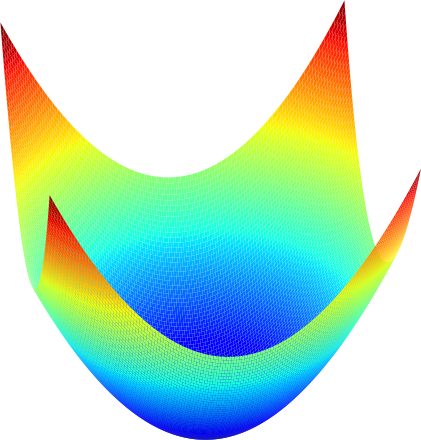
\includegraphics[scale=.4]{Imagenes/smoothvalley.png}
    \caption{Paisaje suave con un gran valle}
\end{subfigure}
    \label{fig:landtypes}
\caption{Diferentes tipos de paisajes de búsqueda. Se muestran paisajes continuos con fines ilustrativos.}
\end{figure}


Las metaheurísticas sirven como una estrategia para explorar el paisaje de búsqueda. Una de las más sencillas e intuitivas es conocida como escalada estocástica y simplemente consiste en reemplazar la solución actual por algún vecino mejor escogido al azar hasta que la solución en la que estemos sea mejor que todos sus vecinos, es decir, un óptimo local. Esta es una metaheurística de trayectoria y traza un camino entre las soluciones inicial y final.

%
\begin{algorithm}[H]
 \KwData{Problema de Optimización}
    \KwResult{Óptimo local $x$}
 Generar solución inicial $x$\;
 \While{$L$ no vacía}{
    Generar lista de vecinos $L$ de $x$\;
    Escoger al azar un vecino $y\in L$\;
  \eIf{$y<x$}{
      $x \leftarrow y$\;
      Generar lista de vecinos $L$ de $x$\;
   }{
       Quitar a $y$ de $L$\;
  }
 }
    \Return{x}
    \label{alg:LS}
    \caption{Algoritmo de escalada estocástica}
\end{algorithm}

\begin{figure}[H]
\centering
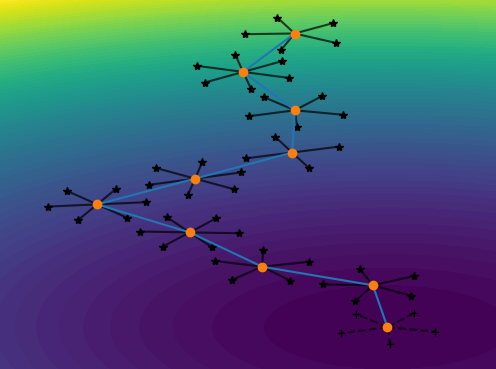
\includegraphics[scale=.7]{Imagenes/mettray.png}
    \caption{Ilustración de una escalada estocástica. Las aristas rayadas representan la vecindad del óptimo local.}
\end{figure}


% introducir ejemplos de mh de trayectoria
Otra metaheurística de trayectoria importante que es parte de muchas de las estrategias que han obtenido los resultados del estado del arte es la llamada búsqueda tabú. Esta metaheurística se basa en la búsqueda local pero puede aceptar vecinos que no mejoran la función de fitness con la intención de evitar atascarse en un óptimo local de mala calidad. La búsqueda tabú almacena soluciones previamente vistas para evitar visitarlas de nuevo. Es necesario definir el tamaño de la lista, el criterio de paro y cómo escoger una nueva solución.\\ 

\begin{algorithm}[H]
 \KwData{Problema de Optimización}
 \KwResult{Mejor solución encontrada $x^*$}
 Generar solución inicial $x$\;
    Inicializar mejor solución como $x^*\leftarrow x$
 Inicializar la lista tabú $TL$ con $x$\; 
 \While{no criterio de paro}{
     Generar lista de vecinos aceptables $L$ de $x$ tal que $L\cap TL =\varnothing$\;
    Escoger un vecino $y\in L$\;
      $x \leftarrow y$\;
      Actualizar $TL$\;
      \If{$x<x^*$}{
      $x^* \leftarrow x$\;
      }
 }
    \Return{$x^*$}
    \label{alg:TS}
    \caption{Algoritmo básico de búsqueda tabú}
\end{algorithm}

\smallskip
Por último se presenta una metaheurística de trayectoria muy sencilla que intenta subsanar el problema de atascarse en óptimos locales de mala calidad de la búsqueda local. La idea es obtener un mínimo local a partir de una solución inicial mediante búsqueda local, aplicarle una perturbación y repetir el proceso hasta que se cumpla algún criterio de paro. Esta estrategia es conceptualmente muy simple aunque se debe definir la perturbación que se hace a la solución y por lo general no es tan sencillo plantear una perturbación adecuada.\\

\begin{algorithm}[H]
 \KwData{Problema de Optimización}
 \KwResult{Mejor solución encontrada $x^*$}
 Generar solución inicial $x$\;
 Inicializar mejor solución como $x^*\leftarrow x$
 \While{no criterio de paro}{
     Obtener una solución $y$ a partir de $x$ mediante búsqueda local \ref{alg:LS}\;
     \eIf{$y<x^*$}{
     $x \leftarrow y$\;
     $x^* \leftarrow y$\;
    }{
     $x \leftarrow x^*$\;
     Perturbar $x$\;
    }
 }
    \Return{$x^*$}
    \label{alg:ILS}
    \caption{Algoritmo búsqueda local iterada}
\end{algorithm}
